% !TeX spellcheck = en_US
% !TEX root = ../thesis-example.tex
%
\chapter{Evaluation \& Future Work}

\section{Hardware Setup Variations}
\label{sec:eval:hardware}

Due to the nature of the setup and fine-tweaking options inside the engine, 
this approach discussed in the previous section can have a wide variety of 
operational setups. By lose coupling of these hardware factors there are only a 
few limitations that can either be solved by better, future hardware or a 
different approach that are outside of the scope.

An integral part of this setup is the motion tracking solution: it is possible 
to hook up an Oculus Rift\footnote{with its room-scale setup} instead of the 
HTC Vive and set one controller as camera-attachment point. For that there 
would be another 3D print needed to attach the controller to a camera solution. 
\newline
Other third market VR-HMDs usually follow the Vive's specifications closely and 
integrate natively with SteamVR, thus no modification on the original 
instalment has to be done.
\newline
Through Virtual Reality Peripheral Network or OpenVR simliar solutions can be 
developed, since none of the software explicitly depends on SteamVR features 
and allow a wide variety of systems and sensors.

The video capturing side can be varied greatly too, since the software only 
requires for webcam-compatible devices, it would be possible to remove 
the Inogeni encoder and replace it with cheap and simple webcams. Similarly, 
can a camera be replaced along with other recording solutions, as long as it 
outputs an HDMI (or HDMI-convertible) video stream. This allows recording to be 
as complex as needed but in general a DSLR camera will suffice.

Finally, since the full pipeline is rather complex, a good desktop PC will be 
needed. The CPU overhead is minimal but the graphical complexity is based on 
limitations of the GPU. With future iteration of this hardware it will be 
possible to create more complex scenery, output higher resolution video and 
better frame rates if the video capture device allows for it.
\newline
In theory, a low-poly environment could be render-able on mobile, combined with 
a low-sample rate on the camera image, to produce a "window" into VR for 
multiple users at the same time, thus enabling an indefinite view into virtual 
reality. This would remove the MR-pipeline from an actor's system. Further work 
could tap into a Microsoft HoloLens solution, which could enable a direct 
contextualization of an actor into a VR scenery without a green screen at all. 
With fast approximate algorithms, like YCgCo-Keying, this could produce a 
high-framerate transparent overlay, so that the virtual scene does not clip the 
actor.

While working with this setup another possible use-case showed up: On June 2017 
Apple presented their native Augmented Reality kit integrated in their consumer 
devices. Thus a similar system could be used to send all tracking parameters 
from the HTC Vive headset to these devices and have a calibrated north-wall 
with additional feature markers. This would potentially allow to have an 
augmented reality view around the actors world with a fast approximated actor 
position. It could then be possible for multiple users to use these devices as 
window into the virtual reality experience without a green screen at all.

\section{Rendering Setup Variations}

There are a few approaches that work similarly, but differ with respect to 
complexity, their capabilities and hardware requirements. They have been 
already explored by producing companies and are covered here for completeness.

\subsection{Single Camera - 3D Plane in Space}

A novel approach is rendering the camera image onto a 2D plane positioned 
inside the 3D scene. This gives high control over projection parameters inside 
the engine without a running software and has good visual feedback for artists. 
All additional steps previously discussed are invalid, since this render can 
take full advantage of all runtime rendering parameters - which in turn means 
for lower render overhead and better graphical performance. It fails however on 
delay mitigation, which makes time drift between engine and camera visible, 
thus only usable with low latency video capturing devices. (Figure 
\ref{fig:alt-render:single-camera} for reference)

\begin{figure}[htb]
	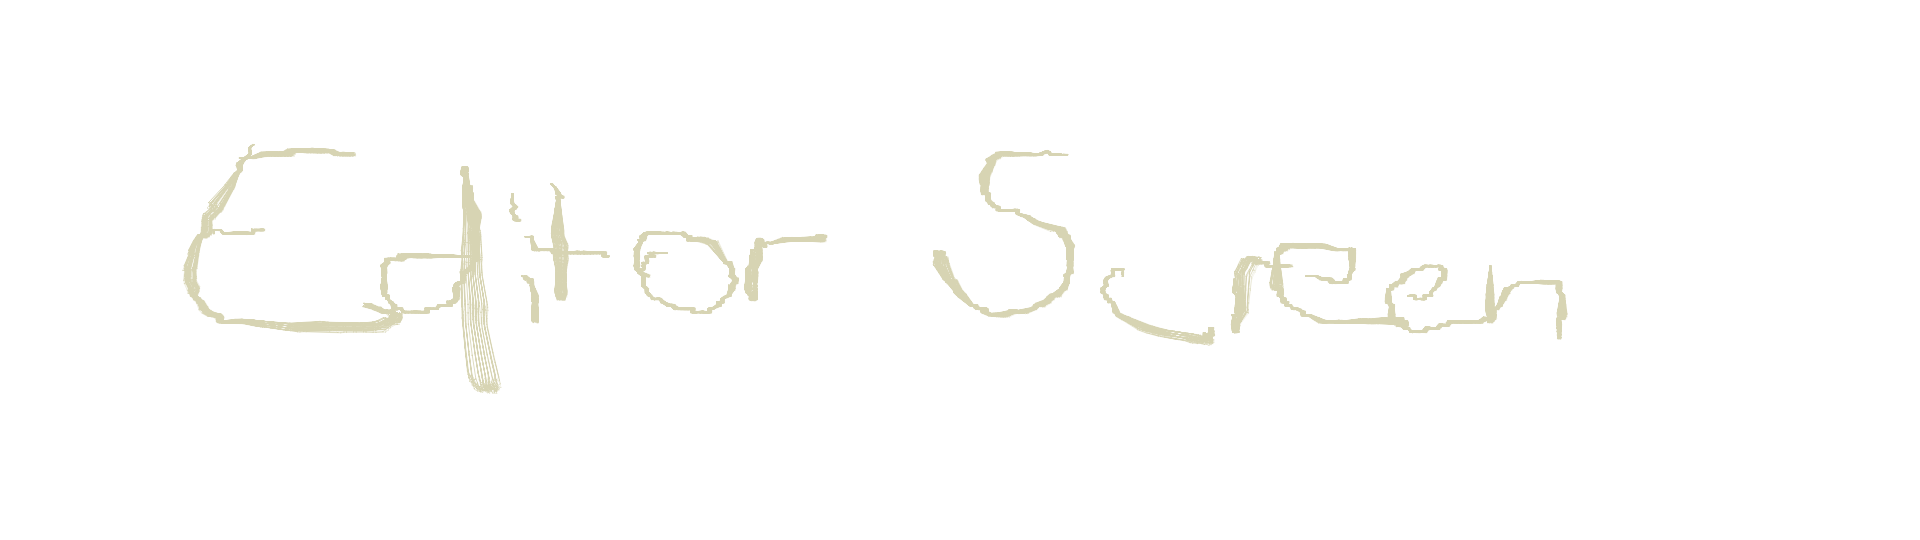
\includegraphics[width=\textwidth]{_raw_resources/editor_single_camera.png}
	\caption{Demonstrative scene with a plane as camera rendering position}
	\label{fig:alt-render:single-camera}
\end{figure}

\subsection{Deferred Shading Path}

Similarly to the single camera approach, a deferred shader could be used, in 
which the plane is projected and texturized after the scene has rendered and 
the graphics buffer is still present - this way the total time taken for 
rendering can be calculated and the chroma keying step can be chosen for a 
faster variant if needed. This gives generally better control and could yield 
higher performance, since all projected fragments have an assigned depth - the 
camera image only has to be calculated where the actor's depth is smaller than 
the scenery's depth. This method is also lacking a way of adjusting for time 
drift. Additionally, calculating lightning is relatively expensive, due to the 
reprojection of lighting parameters inside the graphics buffer. A snapshot of 
this buffer cannot be stored - which is a limitation of Unity's render pipeline 
- and is lost after the rendering loop is completed.

\subsection{Composition Workstation (4 patch)}

Lastly, for full video production setups another rendering approach has been 
suggested, which has been used for the initial promo material for the HTC 
Vive\cite{valve:vive-trailer:2016}. It includes rendering a 4K video signal, 
outputting it to a composition PC which then takes care about managing time 
drift and video input from the camera.
\newline
The general concept involves a production of four 1920x1080 video signals of 
the virtual environment:
\begin{my_list}
	\item Foreground
	\item Video matte of foreground
	\item Background
	\item First person view
\end{my_list}

\begin{figure}[htb]
	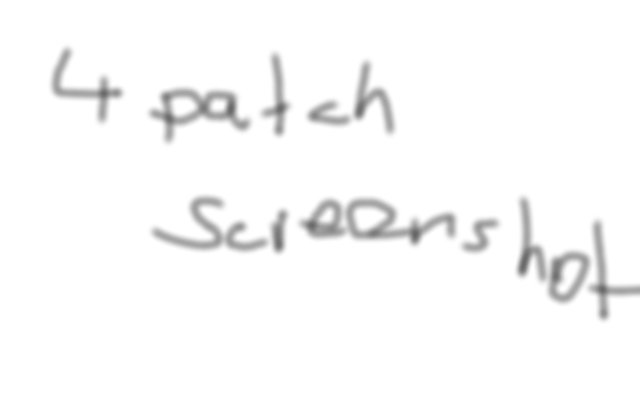
\includegraphics[width=\textwidth]{_raw_resources/4patch_composite.png}
	\caption{Actual order of computation}
	\label{fig:alt-render:4patch}
\end{figure}

Due to the system separation it is now possible to use green screen hardware 
compositors which have a visually higher quality in pulling the green 
background matte and then compositing it similarly into a mixed reality image. 
While this lifts some rendering overhead from the host PC, it fails in 
recreating a lightning environment for the VR actor and relies on two systems. 
While engine programming complexity decreases, operational setup complexity 
increases.

\section{Rendering Operational Variations}

This setup can handle another operational context by leaving out 
background-sorting and only rendering a virtual "front", by which a high 
quality augmented camera system can be achieved. Since time drift between 
camera and engine is already handled, it is possible to render an augmented 
image. Since depth information is lost, it is not possible to handle 
obstructions - for example by an interacting user that is standing in front of 
the augmented object. However, with some composition and choreography, AR 
footage can be showed and captured in live production for further use. A 
reference plane has to be used, either by a Vive Tracker\footnote{like a 
controller} or with feature markers.
\newline
This thesis assumes that the motion video feed is calibrated for a D65 white 
and augmented reality scenarios usually do not take real-world lightning into 
account, it would give a good natural and high quality look into augmented 
reality use cases.

\section{Edge Cases}

The proposed method has edge cases which could be further improved by other 
approaches in rendering or capturing actor video. These highlight issues 
observed with the rendering operations discussed in this thesis.

\subsection{Image Clipping - Incorrect Z Calculation for Hands}

Due to the planar projection of the real world feed inside the engine, any 
Z-information of the actor is squashed to a fixed depth. This means that hands 
are on the same plane. In cases with high z-difference between actor and 
actor's hands, it is possible that hand motion look unnatural and does not seem 
like it is to be supposed - in figure \ref{fig:edge:z-clipping} is an actor 
depicted, whose hands are clearly in front of a virtual cube. The produced 
mixed reality image shows his arms only behind the cube.

\begin{figure}[htb]
	\centering
	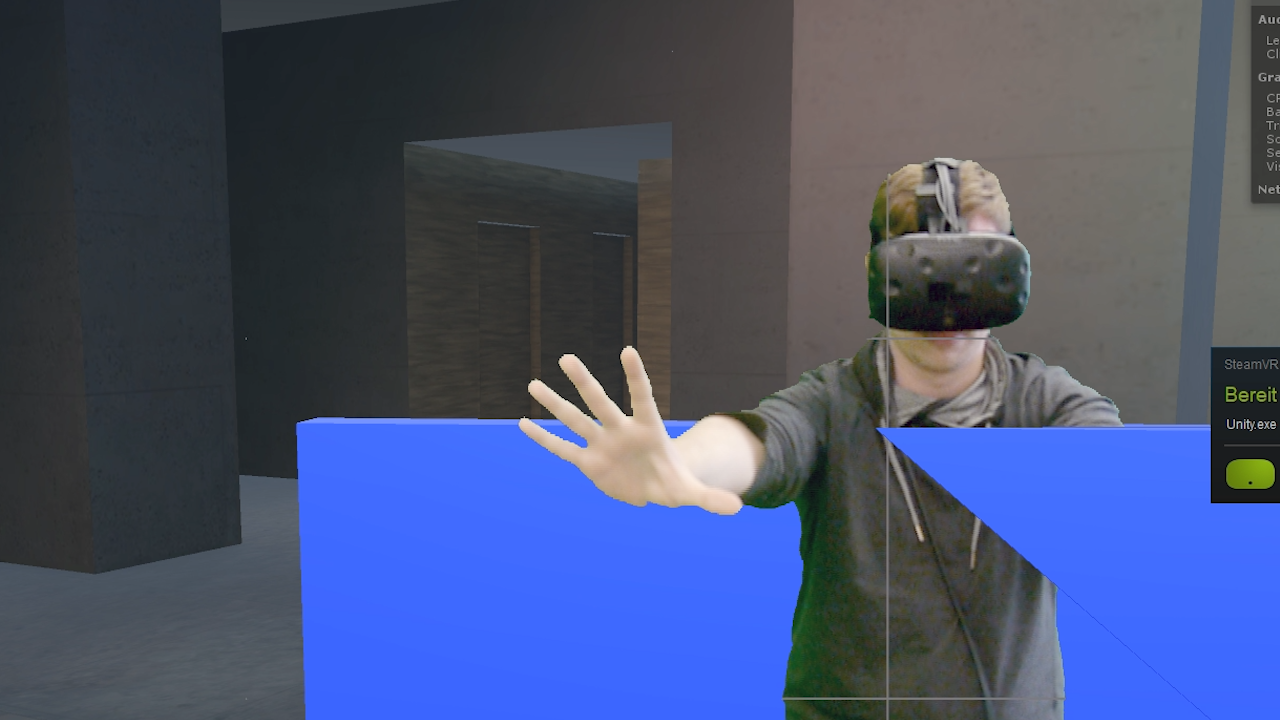
\includegraphics[width=\textwidth]{gfx/issues/z-clipping.png}
	\caption{The actors hands do not visibly reach through the blue cube and 
	the actor shears it because of the planar projection}
	\label{fig:edge:z-clipping}
\end{figure}

One solution for future research could be acquiring an actor's depth by either 
using Time of Flight cameras and using a resulting point cloud or by 
calculating each camera pixel's depth with a stereoscopic solution. Thus each 
pixel could have a quantifiable depth with additional calibration parameters 
from the virtual reality tracking solution.

\subsection{Matting Failures}

There are multiple problems with green screens, which are as old as green 
screens are used in video production. First and foremost is a partial 
transparent actor if his clothing consists of similarly green shaded material.
\newline
Additional green screen spill causes artifacts while pulling the matte which 
then clips the actor off. This can be mitigated by better production 
environments, i. e. with higher quality cloth and a generally well lit 
set\footnote{The appendix features a basic schematic of a small green screen 
setup.}.
\newline
Sometimes, for example in low light environments or folded green screen 
material, the background covers a wide color range, thus calibrating a good 
green with a single color value is nearly impossible. This could be solved by 
smaller selection margins inside the shader while assigning an array of colors 
for the $\Delta E$ calculation. In turn, this would be even more taxing on the 
GPU, since the calculation has be done per selected color, multiplying the 
effort by the number of colors.
\newline
Lastly, real time chroma keying has problems with motion blur of the source 
video material - causing background mixing and invalid matting. This is a 
complex problem that is far beyond the scope of this thesis. One of the best 
solutions is a color unmixing approach researched by Disney and "typically 
requires 10s for local color estimation (assuming 8 dominant colors), another 
second to propagate the local color model to the following frame, and 
approximately 3s for color unmixing." \cite{disney:unmixing:2017}
\todo{Add graphics depicting each issue. Also cross reference to chapter 4}

\subsection{Calibration Problems}

The biggest margin of error is calibration of all projection parameters.
\newline
Beginning from field of view calculation, most DSLR cameras don't have 
specifications for their output feeds, where, for example, scaling factors 
could change the field of view angle. If these are not given or seem to be 
unfitting in production it is necessary to measure these parameters by hand, 
fixing the cameras position and calculating the spanning angle.
\todo{maybe add the ez calculation, too}
Another factor are offset-parameters between controllers and camera sensor, 
which have been minimized by the 3D printed attachment. However, minimal 
differences in this transformation matrix have tremendous impact on 
miscalculated projections, visible by wrongly placed objects and a disconnect 
between virtual interaction and actor.
\todo{Here comes a graphical representation of it}
Lastly, the most time spent after adding all mixed reality components to the 
scene is calibrating these parameters. A possible improvement could be done by 
fixing the cameras position, showing an overlay on the camera, where the 
secondary controller has to be placed and confirming it. This way the user can 
calibrate all projection parameters by himself with the help of a RANSAC / 
Lagrange Polynomial.
\todo[inline]{find out how this calibration is called: 
https://www.youtube.com/watch?v=c\_An0vxvPnk}